\documentclass[twocolumn]{Jornadas}
\usepackage[utf8]{inputenc}
%\usepackage[dvips]{graphics}
\usepackage[pdftex]{graphicx}
%\usepackage{epsfig}
\usepackage[spanish]{babel}
\usepackage{subfig}

\def\BibTeX{{\rm B\kern-.05em{\sc i\kern-.025em b}\kern-.08em
    T\kern-.1667em\lower.7ex\hbox{E}\kern-.125emX}}

\newtheorem{theorem}{Teorema}

%%%%%%%%%%%%%%%%%%%%%%%%%%%%%%%%%%%%%%%%%%%%

%\hyphenation{}

\begin{document}

\title{Análisis de la Carga de Trabajo de un Servidor Proxy}

\author{%
     Salvador Climent Bayarri, %
     Andrew Fecheyr-Lippens, %
     Alejandro Valero Bresó%
	\thanks{Máster en Ingeniería de Computadores, Universidad Politécnica de Valencia, e-mails: {\tt jocliba@upvnet.upv.es, fecanfra@posgrado.upv.es, alvabre@gap.upv.es}}
     }

\maketitle
% Oculta las cabeceras y los números de página.
% Ambos elementos se añadirán durante la edición de las actas completas.
\markboth{}{}
%\pagestyle{empty}
\thispagestyle{empty} % Oculta el número de la primera página

\begin{abstract}

La técnica de caching consiste en almacenar objetos en caches cercanas a los clientes que los solicitan. Los aciertos en la cache eliminan la necesidad de acceder al servidor, reduciendo notablemente la demanda de ancho de banda, la latencia y el tráfico de la red a la vez que se mejora la disponibilidad del servidor. Esta técnica se puede evaluar mediante la caracterización de la carga, ya que explota propiedades específicas de los accesos para mejorar las prestaciones. Mediante la caracterización de un sistema en el tiempo se pueden observar los cambios que el sistema ha sufrido.

Este artículo presenta un estudio detallado de la caracterización de la carga de trabajo de un servidor proxy. En concreto, se analizan características como la eficiencia del servidor proxy, los códigos de respuesta del proxy, los tipos de objetos, el tamaño de los objetos únicos y solicitados, la evolución de la carga del proxy durante el día, la localidad temporal y el tiempo de sesión de los usuarios.

\end{abstract}

%\begin{keywords}

%\end{keywords}

\section{Introducción}
\label{intro}

\PARstart{L}{a} popularidad del \emph{World Wide Web}, específicamente el alto porcentaje del tráfico HTTP, es una de las principales razones por las que el tráfico en Internet se ha incrementado con los años. Para entender este incremento del tráfico, podemos destacar las cifras de principios de los años 90. Los estudios mostraban que el 44\% del tráfico en Internet era originado por peticiones FTP, mientras que durante los primeros años del nuevo milenio, entre un 75 y un 80\% del tráfico en Internet está formado por la actividad HTTP \cite{barish}. Este incremento del tráfico en Internet lleva asociada la demanda de escalabilidad en su infraestructura. El crecimiento exponencial de la Web desprovisto de soluciones escalables resulta en una carga en la red prohibitiva y unos tiempos de respuesta inaceptables. Además, el uso de la Web forma parte de la vida rutinaria y los negocios de las personas, con lo que las mejoras de las prestaciones en la Web es un hecho deseable, pero sobre todo necesario.

El presente estudio comprueba que la gran mayoría (tanto en número de peticiones como en bytes transmitidos) de los objetos HTTP demandados por los usuarios son imágenes y código HTML. Con vistas al futuro, el hecho de incluir la etiqueta de vídeo en el nuevo estándar HTML5 y la posibilidad de realizar HTTP Streaming, nos hace pensar que los vídeos podrán llegar a ser una parte importante del tráfico HTTP.

Existen diversas técnicas para mejorar las prestaciones de la Web. Las páginas Web pueden hacer uso de clusters para manejar las peticiones de los clientes. Por otra parte, se pueden mejorar los enlaces de la red para conseguir mayor ancho de banda y así manejar el volumen creciente de los datos que se transfieren. Sin embargo, estas técnicas representan soluciones a corto plazo. El crecimiento de Internet en términos del número total de bytes transmitidos entre las máquinas y el inesperado uso masivo del protocolo HTTP, hacen de la técnica de Web caching la solución más atractiva y la que más atención ha recibido. Se trata de una de las técnicas más importantes de reducción de tráfico en la red.

Esta técnica consiste en almacenar documentos en caches cercanas a los clientes que los solicitan. Los aciertos en la cache eliminan la necesidad de contactar con el servidor, con lo cual representa una forma efectiva de reducción de la demanda de ancho de banda, mejora de la disponibilidad del servidor Web (evita que se convierta en un \emph{hotspot}) y reducción de la latencia de la red.

La técnica de caching puede mejorar la percepción que tienen los usuarios en cuanto a las prestaciones de la red. Cuando sirven a los clientes localmente, las caches ocultan la latencia resultante de las redes de gran tamaño. Cuando se produce un fallo local de cache, el proveedor original sirve las peticiones de los clientes.
Este hecho cobra gran importancia con los objetos de naturaleza temporal (datos multimedia como audio o vídeo) donde mantener una tasa de transferencia constante y el tiempo de respuesta son particularmente importantes.

\subsection{Caracterización de la carga}
Los beneficios de la técnica de caching han sido demostrados mediante algunos prototipos de investigación y la experimentación con grandes niveles de caching en la Web \cite{squid}. 

La caracterización de la carga es importante porque la técnica de caching explota propiedades específicas de los accesos para mejorar las prestaciones como la localidad temporal. Además, es una componente crucial del diseño de sistemas debido a que permite entender el estado actual del sistema y observar posibles cambios.

En la bibliografía existen multitud de artículos referentes a la caracterización de la carga. Podemos referenciar algunos artículos que presentan cierta similitud con nuestro análisis de la carga como la caracterización de la carga de Arlitt et al. \cite{arlitt2} y Mahanti et al. \cite{mahanti}.

El resto del artículo se organiza de la siguiente manera: la Sección \ref{meto} muestra como se distribuyen los datos contenidos en logs de acceso y como se lleva a cabo la reducción de datos. La Sección \ref{resultados} presenta el estudio de la caracterización de la carga. Finalmente, la Sección \ref{conclusiones} ofrece las conclusiones más relevantes.

\section{Metodología}
\label{meto}

Los logs de acceso del servidor proxy fueron recogidos en la Universidad Politécnica de Valencia entre los días 16 de febrero de 2009 y 3 de marzo de 2009, con lo que se obtuvo un contenido total de logs de acceso de 23GBytes. Antes de realizar el procesamiento de los logs, resulta necesario interpretar los datos contenidos en las entradas de los mismos, así como reducir la cantidad de datos eliminando las entradas incorrectas que afectan a la caracterización de la carga y los datos no relevantes para reducir el tiempo de procesado de la carga. Esta sección trata estos aspectos.

\subsection{Interpretación de los logs}

Cada entrada de un log de acceso contiene información de una sola petición de un cliente recibida por el proxy Web. Con esto, una entrada contiene la siguiente información:

\begin{description}
\item[Timestamp] El momento en el que una petición ha sido completada.
\item[Elapsed] Considera el número de milisegundos en los que la transacción ha ocupado la cache.
\item[Remotehost] La dirección IP del cliente.
\item[Code/status] Consta de dos entradas separadas mediante una barra. Almacena el resultado de la transacción. Consultar la lista de códigos, que detallaremos a continuación, para obtener los posibles valores.
El estado es un número asociado al código.
\item[Bytes] El tamaño de los datos enviados al cliente.
\item[Method] El método de petición para obtener un objeto.
\item[URL] Este campo contiene la URL solicitada por el cliente.
\item[rfc931] No se utiliza por problemas de rendimiento.
\item[Hierarchy code] Información de herencia de las caches. En el caso que nos ocupa solo tenemos un servidor de cache, así que los fallos de cache siempre se enviarán al servidor Web. 
\item[Content type] Consiste en el tipo de objeto tal y como se especifica en la cabecera de respuesta HTTP.
\end{description}

La siguiente lista muestra los posibles códigos asociados a cada entrada de un log de acceso:

\begin{description}
\item[TCP\_HIT] Una copia válida del objeto solicitado se encuentra en la cache y es leída del disco.
\item[TCP\_MEM\_HIT] Una copia válida del objeto solicitado se encuentra en la cache y en memoria, así que no debe ser leída del disco.
\item[TCP\_NEGATIVE\_HIT] La petición se realiza sobre un objeto \emph{negativamente-cacheado}. El cacheado negativo se refiere a cachear ciertos tipos de errores, como \emph{404 Not Found}. El parámetro de configuración \emph{negative\_ttl} controla la cantidad de tiempo de cacheo de estos errores.
\item[TCP\_MISS] El objeto solicitado no se encuentra en la cache.
\item[TCP\_REFRESH\_HIT] Una copia del objeto solicitado que ha expirado se encuentra en la cache. Squid realiza una petición \emph{If-Modified-Since} y la respuesta es \emph{Not Modified}.
\item[TCP\_REFRESH\_FAIL\_HIT] Una copia del objeto solicitado que ha expirado se encuentra en la cache. Squid realiza una petición \emph{If-Modified-Since} pero ésta provoca un fallo. La copia vieja (caducada) del objeto se envía al cliente.
\item[TCP\_REFRESH\_MISS] Una copia del objeto solicitado que ha expirado se encuentra en la cache. Squid realiza una petición \emph{If-Modified-Since} y recibe una copia nueva de un objeto diferente.
\item[TCP\_CLIENT\_REFRESH\_MISS] El cliente emite una petición con el pragma \emph{no-cache} (\emph{Recarga} - manejada como un fallo)
\item[TCP\_IMS\_HIT] Una petición \emph{If-Modified-Since GET} es recibida del cliente. Una copia válida del objeto (fresca) se encuentra en la cache.
\item[TCP\_IMS\_MISS] Una petición \emph{If-Modified-Since GET} es recibida del cliente. El objeto solicitado no se encuentra en la cache (caducado).
\item[TCP\_SWAPFILE] Se pensaba que el objeto se encontraba en la cache, pero no puede ser accedido.
\item[TCP\_DENIED] Acceso denegado para la petición.
\end{description}

\subsection{Reducción de datos y procedimiento}
\label{red_datos}

Para poder procesar eficientemente la información, los logs de acceso los hemos insertado en una base de datos MySQL.

Esta inserción de datos en la base de datos se ha realizado teniendo en cuenta pequeñas optimizaciones para facilitar el procesamiento de los datos y son: i) eliminar la columna \textit{rfc931} ya que esta funcionalidad no se utiliza en el proxy y siempre presenta el mismo valor, así como la columna \textit{hierarchy code} porque sólo hay un proxy en nuestro escenario, ii) utilizar  enumeraciones en las columnas action, method y content type y iii) almacenar la dirección IP como un entero utilizando la función INET\_ATON() de MySQL.

Además de estas optimizaciones, también hemos eliminado de los logs los objetos que hemos visto que no son cacheables. Para ello, hemos realizado una búsqueda de diferentes subcadenas en las URL y hemos comprobado si se producían aciertos de cache para esos objetos. Solo hemos eliminado aquellas URLs que coincidían con la subcadena '.cgi?' ya que ninguna de estas url producía aciertos en la cache y, por tanto, hemos supuesto que eran objetos no cacheables.

Por otra parte, en los análisis de datos previos que realizamos, encontramos que había ciertos datos anómalos en los logs, provocando comportamientos puntuales y extraños en la caracterización de la carga. Estos datos anómalos podrían resultar inapreciables si el periodo de recogida de datos hubiese sido más largo, pero al contar con solo 15 días de logs afectaban de manera apreciable a los resultados y decidimos descartarlos para realizar el análisis.

Las URLs que han sido filtradas, así como el número de peticiones y el tamaño total se muestran en la Tabla \ref{table:url}. El objeto \textit{favicon.ico} fue descargado por un una IP concreta durante una noche dos millones y media de veces y afectaba sobretodo al análisis de la evolución de la carga del servidor durante el día, con lo que decidimos descartarlo. Por otra parte, también descartamos las entradas con peticones al fichero \textit{video.mjpg} ya que se realizaban a un servidor con IP local. Las últimas dos filas de la tabla hacen referencia a los objetos \textit{.cgi?} que descartamos por ser no cacheables.

Con el filtrado de estas URLs el volumen total de los logs de acceso se reduce en un 3.5\%.

\begin{table*}[ht!]
\centering
\renewcommand{\baselinestretch}{1.5}
\scriptsize
%\tiny \footnotesize
\begin{tabular}{|l||c|c|} \hline
URL Filtrada                                  & Peticiones & Tamaño Total Peticiones (GB) \\\hline\hline
http://muchachadanui.rtve.es/favicon.ico      & 2423780    & 1.7                          \\\hline  
http://172.18.18.71/mjpg/video.mjpg           & 400        & 314.4                        \\\hline 
http://172.18.18.72/mjpg/video.mjpg           & 320        & 190.1                        \\\hline 
http://172.17.69.324/axis-cgl/jpg/Image.cgi?  & 5300740    & 94.5                         \\\hline 
Otros .cgi?                                   & 208960     & 1.4                          \\\hline 
\end{tabular}
\caption{URLs Filtradas}
\label{table:url}
\end{table*}


\section{Caracterización de la Carga}
\label{resultados}

En esta sección presentamos los resultados de nuestro trabajo de caracterización de la carga. La sección se divide en varios apartados según el análisis trate la eficiencia del servidor, los códigos de estado, los tipos de objetos, el tamaño de los objetos únicos y solicitados, la evolución de la carga del servidor durante el día, la localidad temporal o el tiempo de sesión de los usuarios.

\subsection{Eficiencia del servidor proxy}\label{eficiencia}
A partir de los logs del proxy podemos extraer información sobre el ancho de banda ahorrado por la universidad al encontrarse los objetos demandados por los usuarios en la cache del proxy. Además, también podemos observar la ganancia en el tiempo de respuesta cuando el objeto está en la cache.

En la Figura \ref{fig:elapsed} se puede observar el tiempo transcurrido en ms para resolver la petición dependiendo del tipo de acierto o fallo de cache. Se aprecia una gran diferencia entre el tiempo necesario para resolver una petición de un objeto que ya está en cache y el tiempo necesario para resolver una petición de un objeto que no está en cache. Por otra parte, así como la diferencia de tiempo transcurrido entre diferentes tipos de fallo de cache es bastante apreciable, la diferencia de tiempo transcurrido para los diferentes tipos de aciertos no es tan significativa.

Esta diferencia no es tan significativa entre los diferentes tipos de acierto porque la diferencia de tiempo de recuperar un objeto de memoria o de disco es muy pequeña comparada con la diferencia entre un acierto y un fallo. Por otra parte, la diferencia de tiempo entre un acierto IMS y uno normal también es muy pequeña ya que la mayor parte del tiempo corresponde al acceso al objeto, no a la transferencia de este por la red (en un acierto IMS no se transfiere una copia del objeto al cliente).

A su vez, en la Figura \ref{fig:ahorrado} se muestra el ancho de banda consumido por el total de las peticiones realizadas al proxy y el ancho de banda no consumido gracias a los aciertos de cache durante el transcurso de los días tomados para obtener los logs. Como se observa, el máximo ancho de banda ahorrado está alrededor de 6 Mbps, que es aproximadamente un 15\% del ancho de banda en los momentos de máxima demanda. También se puede observar como el ancho de banda ahorrado es prácticamente nulo en los momentos de más baja demanda. Veremos esto con más detenimiento en la Sección \ref{cargaDia}.

\begin{figure}[ht!]
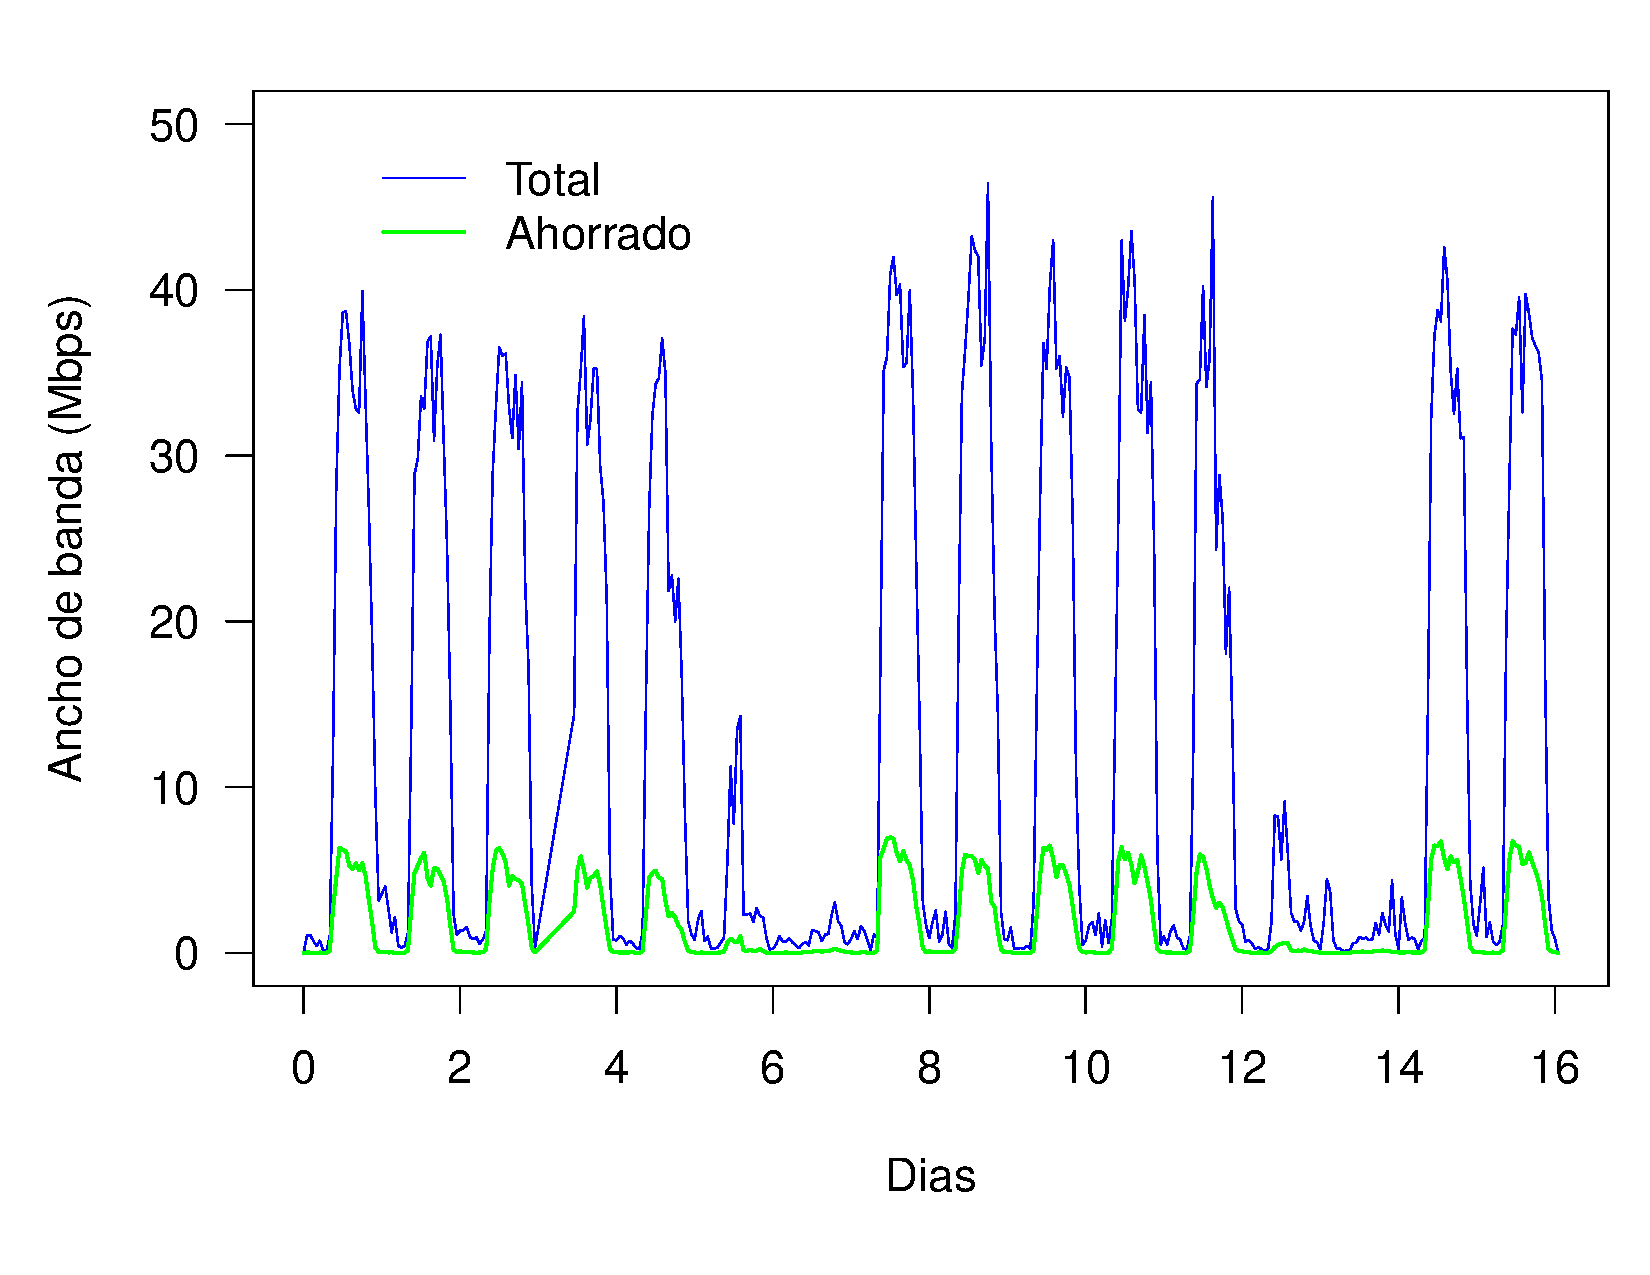
\includegraphics[scale=0.29]{figures/Bandwidth_full.pdf}
\caption{Ancho de banda total y ahorrado}
\label{fig:ahorrado}
\end{figure}

\begin{figure}[ht!]
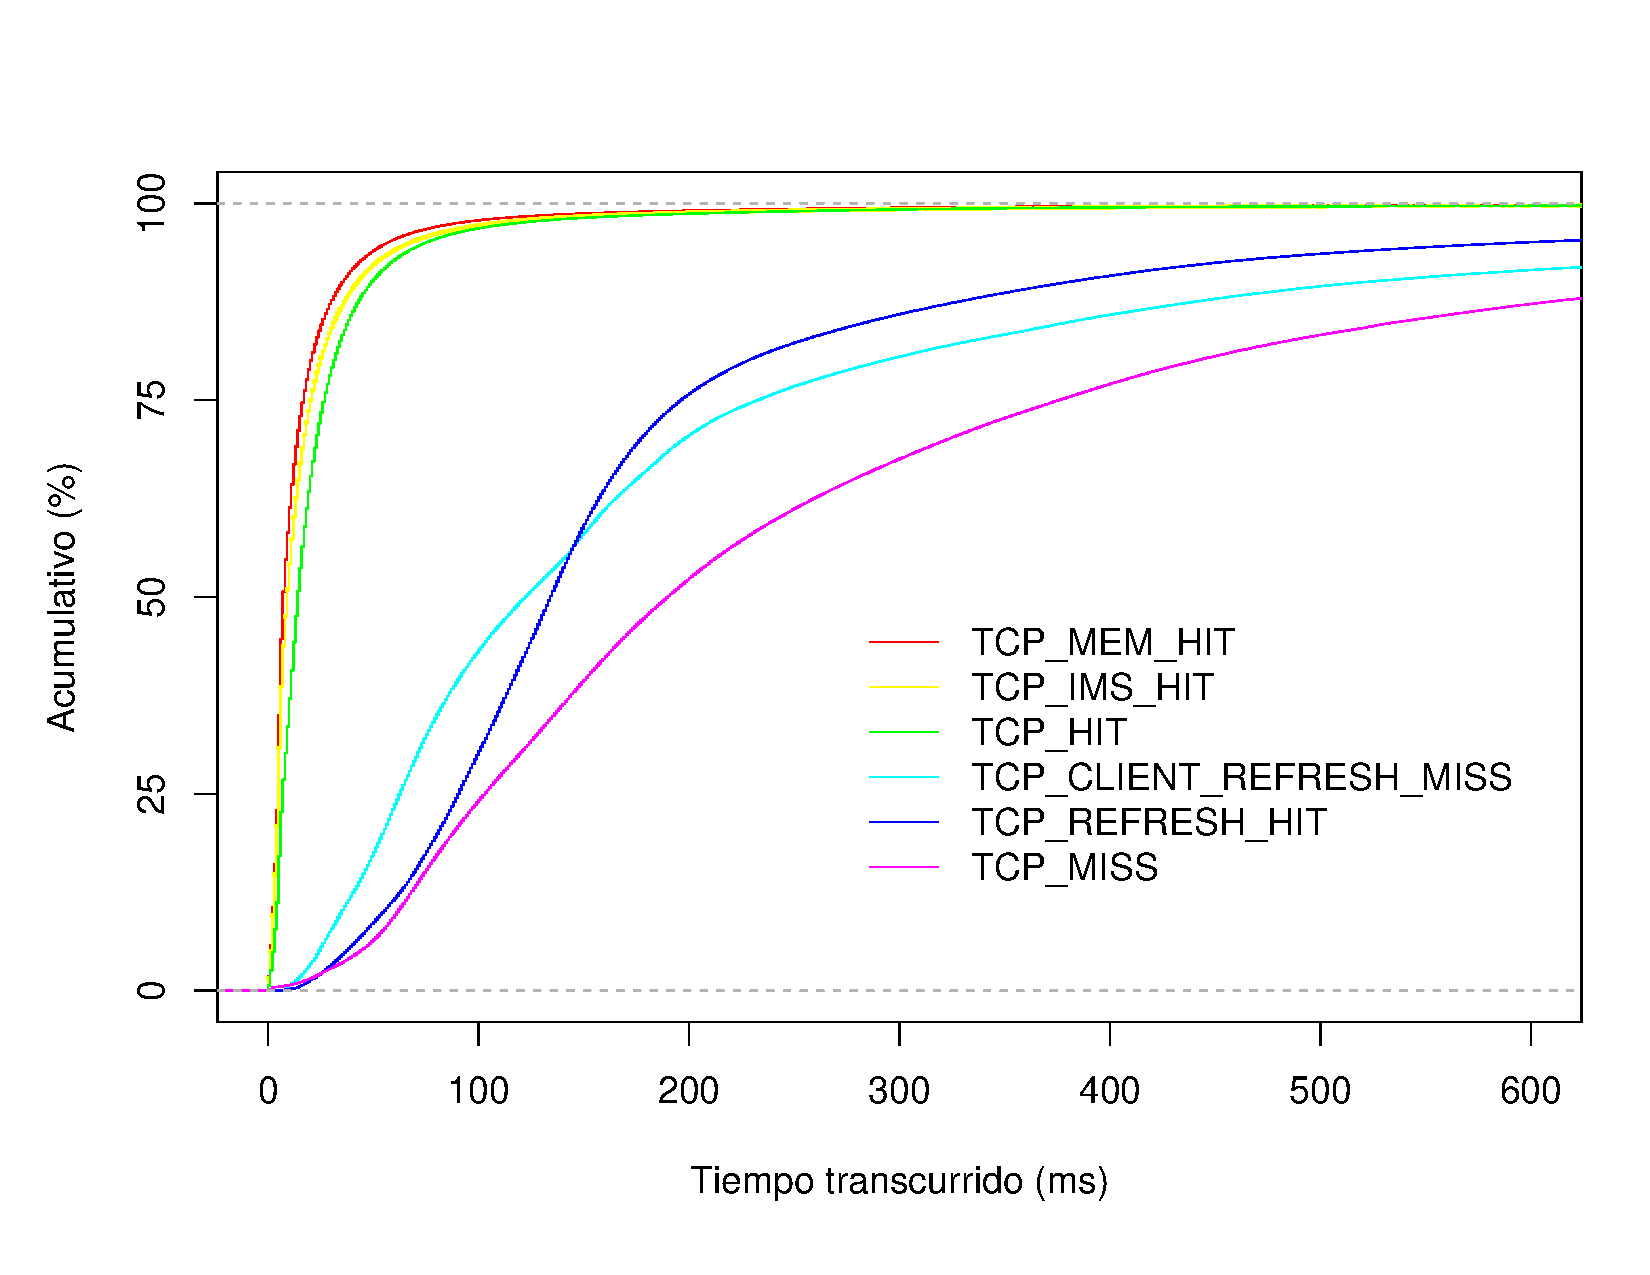
\includegraphics[scale=0.30]{figures/ElapsedTimeAll_1k_full.pdf} 
\caption{Tiempo necesario para resolver una petición dependiendo del tipo de acierto/fallo de cache}
\label{fig:elapsed}
\end{figure}

\subsection{Códigos de estado}
En esta sección analizamos los códigos de respuesta del proxy. La Tabla \ref{table:codigos} muestra los posibles códigos. La mayoría de las peticiones de los clientes (68\%) terminan siendo satisfactorias y además, estas respuestas se corresponden a la mayoría de datos transferidos. La siguiente respuesta más común es \textit{Not Modified} con un 19\% de todo el tráfico HTTP pero, como esperábamos, no tienen impacto en los datos transferidos porque sólo se transfieren las cabeceras HTTP al no haberse modificado el objeto.

\begin{table*}
\centering
\renewcommand{\baselinestretch}{1.5}
\scriptsize
%\tiny \footnotesize
\begin{tabular}{|l||c|c|c|c|c|c|c|} \hline
  & Satisfactorio (200) & No Modif. (304) & Encontrado (302) & No Encontrado (404) & No Content (204) &Otros\\\hline\hline
Peticiones (\%)    & 68.20  & 19.41 & 2.86 & 1.02 & 0.78 & 7.73            \\\hline  
Datos (\%)        & 95.37   & 0.34 & 0.15 & 0.12 & 0.02 & 4.98             \\\hline 
\end{tabular}
\caption{Códigos de estado}
\label{table:codigos}
\end{table*}


\subsection{Tipos de objetos (MIME)}
\label{mime}

\begin{table}
\centering
\renewcommand{\baselinestretch}{1.5}
\scriptsize
%\tiny \footnotesize
\begin{tabular}{|l||c|c|c|} \hline
Contenido   & Peticiones & Peticiones (\%) &Tam. Total (GB) \\\hline\hline
Imágenes    & 80339008   & 51.40 &483             \\\hline  
HTML        & 39663602   & 25.59 &200             \\\hline 
Javascript  & 16893965   & 10.90 &106             \\\hline 
Flash       & 14947413   & 9.65 & 100              \\\hline 
Doc.       & 2727847    & 1.76 &49              \\\hline
Vídeo       & 180369     & 0.12 & 559             \\\hline 
Audio       & 128793     & 0.08 & 115             \\\hline 
Otros       & 85729      & 0.06 & 661             \\\hline\hline
Total & 154966726 & 100 & 2273 \\\hline
\end{tabular}
\caption{Tipos de objetos solicitados}
\label{table:contenido}
\end{table}

En este apartado hemos analizado los tipos de objetos que han demandado los clientes.
Estos objetos se pueden clasificar en las siguientes categorías según su contenido: imágenes, HTML, javascript, flash, documentos, vídeo, audio y otros.
Esta clasificación ha se llevado a cabo mediante la etiqueta \emph{Content Type}. En concreto, los objetos incluidos en las categorías de imágenes, audio y vídeo se corresponden con los \emph{Content Type} que empiezan por \textit{image/}, \textit{audio/} y \textit{video/} respectivamente.
Por su parte, la categoría HTML está formada por objetos cuyo \emph{Content Type} incluye las cadenas \textit{html}, \textit{css} o \textit{text/xml}.
La categoría javascript contiene objetos cuyo \emph{Content Type} es \textit{javascript}. La categoría flash cuenta con objetos con un \emph{Content Type} como \textit{flash}, \textit{flv} o \textit{shockwave}. En la categoría documentos se incluyen los objetos que se corresponden con un \emph{Content Type} como \textit{pdf}, \textit{doc}, \textit{xls}, \textit{word}, \textit{excel} o \textit{powerpoint}. Por último, los objetos clasificados en la categoría de otros cuentan con un \emph{Content Type} diferente a los anteriores.

La Tabla \ref{table:contenido} muestra los diferentes tipos de objetos solicitados al servidor proxy. Como cabía esperar, los objetos clasificados como imágenes son los que mayor número de peticiones generan, sobrepasando el 50\% del total de las peticiones. En segundo lugar aparecen los objetos HTML, que suponen alrededor de un 26\% del total de peticiones. Sin embargo, las imágenes y los HTML representan un 21 y un 9\% sobre el tamaño total en GB de las peticiones. Este efecto se debe a la presencia de vídeos y audios que ocupan mayor tamaño respecto a una imagen y un HTML.   

\subsection{Tamaño de los objetos únicos y solicitados}
\label{unicos_solicitados}

\begin{figure*}[ht!]
\centering
\subfloat[]{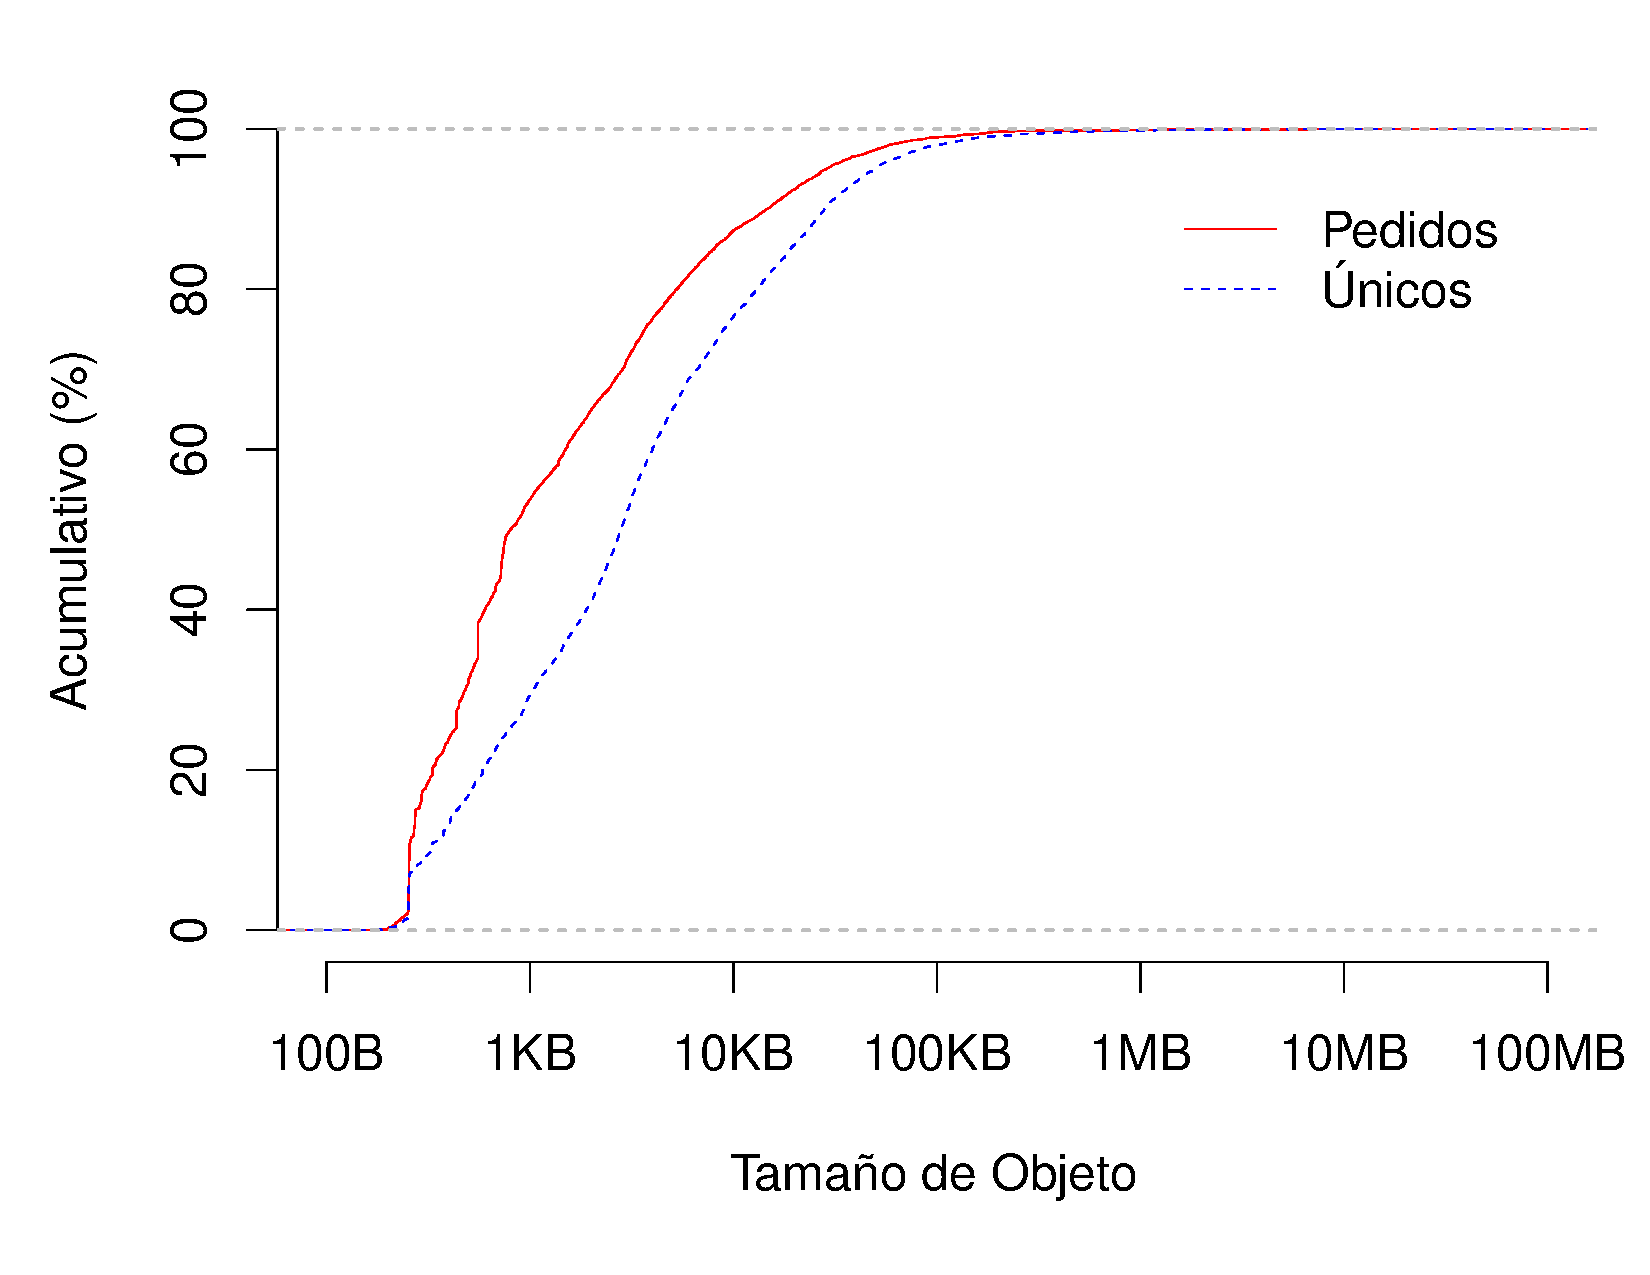
\includegraphics[scale=0.30]{figures/ObjectSizeCumulative_full.pdf}\label{Acumulativo}}
\subfloat[]{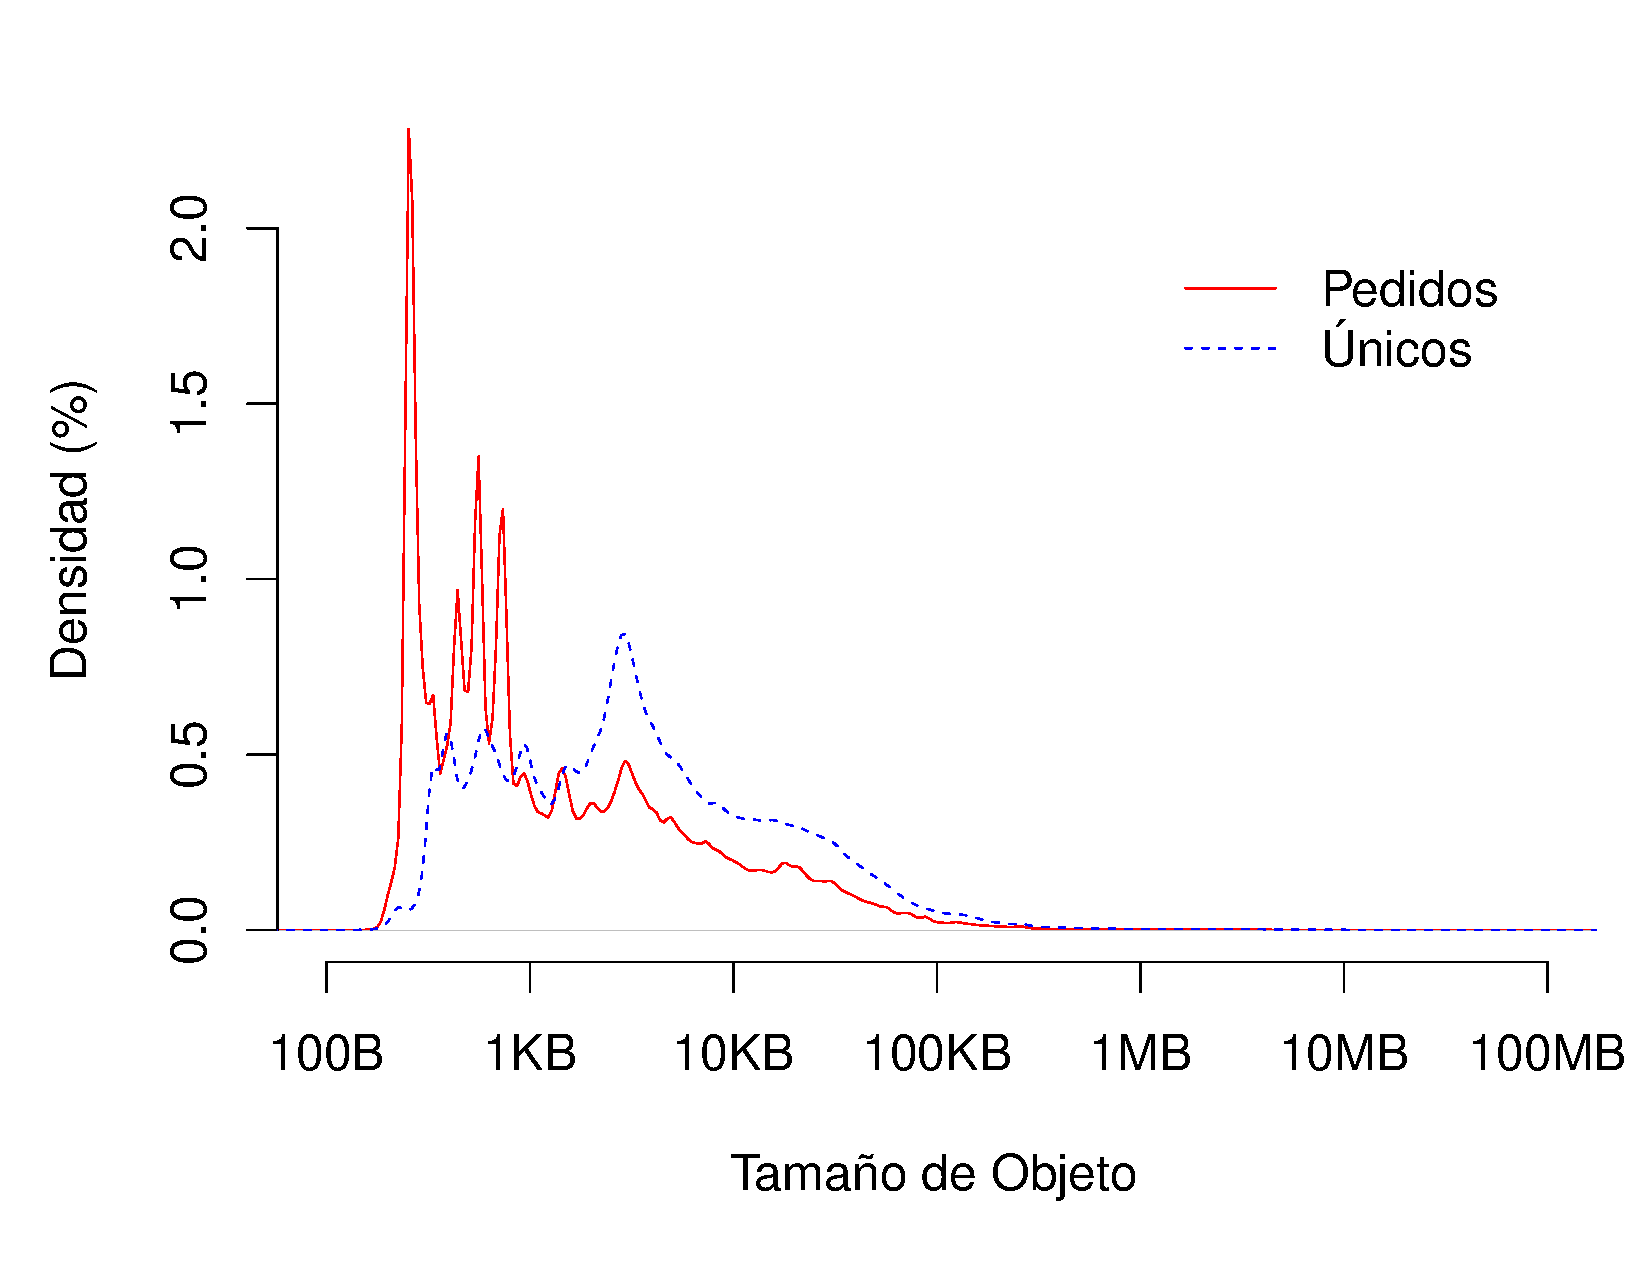
\includegraphics[scale=0.30]{figures/ObjectSizeDensity_full.pdf} \label{Densidad}}
\caption{Análisis de la distribución del tamaño de los objetos únicos y solicitados}
\label{fig:tamObjetos}
\end{figure*}

Para estudiar el tamaño de los objetos, obtenemos resultados acumulativos y de densidad según el tamaño de los objetos que han sido requeridos.
Además, realizamos una distinción entre objetos solicitados y únicos.
Los objetos solicitados conforman todas las peticiones a objetos que realiza el cliente, aunque se solicite el mismo objeto varias veces. Por otra parte, los resultados de los objetos únicos son aquellos que sólo tienen en cuenta la primera referencia a un objeto concreto, descartando el resto.

La Figura \ref{Acumulativo} muestra la distribución acumulativa del tamaño de los objetos solicitados al servidor proxy.
Téngase en cuenta que el eje X es logarítmico, con lo que pequeños incrementos en la pendiente suponen un crecimento significativo.
Estudios previos \cite{arlitt2}\cite{crovella} muestran que el tamaño de los objetos se expande varios órdenes de magnitud, desde decenas de B hasta decenas de MB.
Estos estudios sugieren que la distribución del tamaño de los objetos sea \emph{heavy-tailed} o de \emph{colas-pesadas}. Una distribución de colas-pesadas tiene la propiedad de que la cola de la distribución (valores a la derecha en la Figura \ref{Acumulativo}) se incrementa lentamente. Esto significa que si tomamos tamaños aleatorios de los objetos, la probabilidad de obtener valores extremadamente grandes no es negligible.

%La distribución es \emph{heavy-tailed} o de colas-pesadas. Una distribución se define como de colas-pesadas si, a pesar de la distribución de los valores pequeños de la variable aleatoria, la forma asintótica de la distribución es hiperbólica. %\textcolor{red}{paper de Mahanti, pag 15}

En nuestro caso, el tamaño de la mayoría de los objetos se encuentra entre 100B y 100KB y podemos observar que la distribución es de colas pesadas.
Por otra parte, la curva de los objetos solicitados se encuentra por encima de la de los objetos únicos. Esto se debe a que los objetos más populares son los de tamaño pequeño y por tanto se generan más peticiones de estos objetos al servidor proxy.

En la Figura \ref{Densidad} podemos observar la distribución de la densidad del tamaño de los objetos, tanto únicos como solicitados, en una escala logarítmica. Se puede observar como ninguna de las dos curvas sigue una distribución predefinida.

\subsection{Evolución de la carga del servidor durante el día}\label{cargaDia}

\begin{figure}[tbp]
\begin{center}
  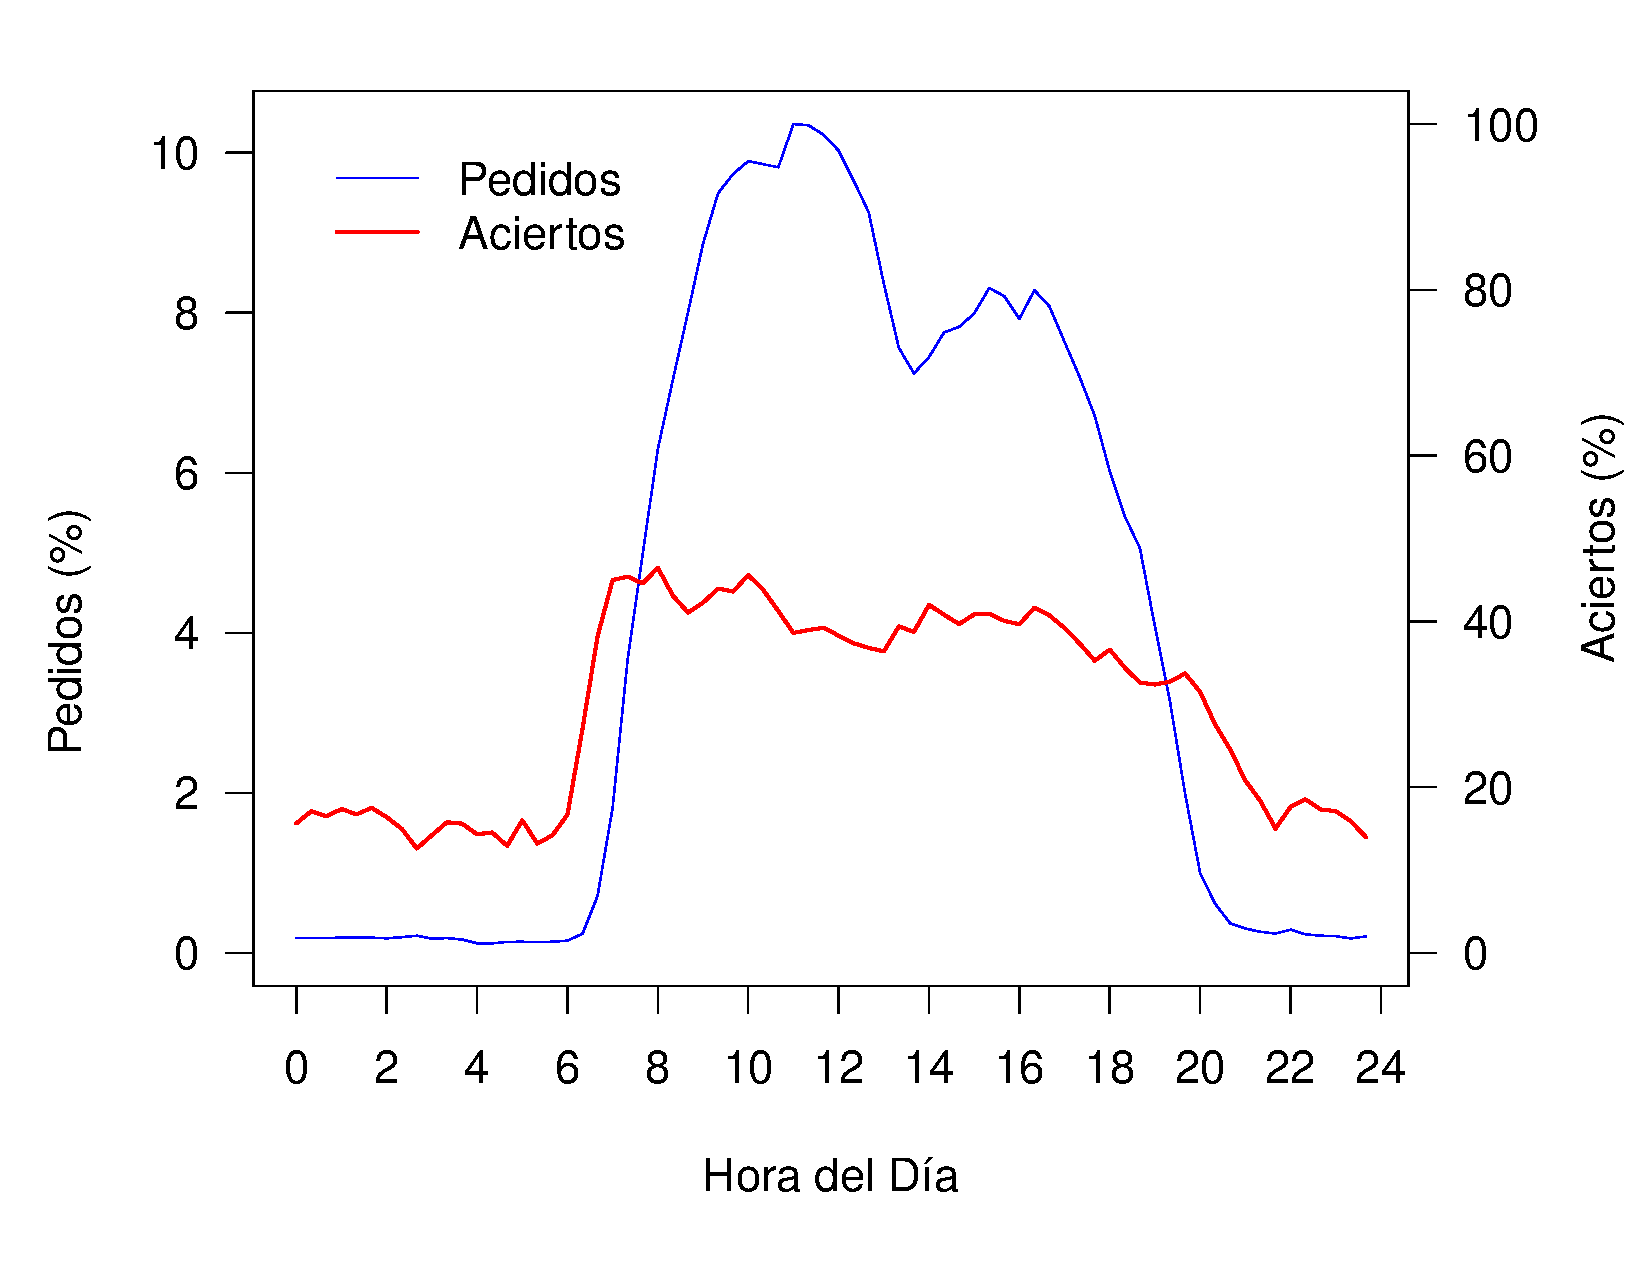
\includegraphics[scale=0.30]{figures/TimeOfDay3_full.pdf}
\end{center}
\caption{Evolución de la carga del servidor durante el dia} \label{Timeday}
\end{figure}

La Figura \ref{Timeday} muestra el análisis de las solicitudes y aciertos según el momento del día. La gráfica se debe interpretar con cautela, ya que la escala para la curva de solicitados llega hasta el 10\% mientras que la curva de aciertos es sobre el 100\%. 

Como se esperaba, en la curva de solicitados podemos observar como la carga resulta baja durante la noche, aumentando durante las horas de la jornada laboral y llegando a su punto máximo a las 12 horas del mediodía. Se puede incluso observar un ligero descenso en las horas de comida (13-15h) y un ligero aumento por la tarde, pero no mayor que durante las horas laborales matinales.

Por otra parte, la curva de aciertos nos muestra como varía la tasa de aciertos con las horas del día. Puede observarse como conforme el número de peticiones aumenta el número de aciertos aumenta hasta que se estabiliza en un valor entre el 30\% y el 40\%.

\subsection{Localidad temporal}



Existe gran cantidad de bibliografía \cite{mahanti},\cite{Breslau},\cite{arlitt2} donde se hace referencia a que algunos objetos en la Web son más populares que otros, es decir, que los patrones de referencia no son uniformes. Teniendo en cuenta esto, hemos llevado a cabo dos análisis para determinar si este comportamiento también está presente en nuestra carga.

El primer análisis se basa en la concentración de referencias entre los objetos únicos y los bytes solicitados. Los objetos únicos se encuentran ordenados en base al número de veces que son requeridos. Para cada uno de estos objetos hemos determinado la fracción de todas las peticiones de los clientes. La Figura \ref{fig:ObjectPopu} muestra los resultados obtenidos y confirma que los patrones de referencia no son uniformes. Podemos distinguir entre tres agrupaciones observando la figura: i) objetos extremadamente populares donde el 1\% de los objetos únicos suponen un 60\% de las solicitudes de los clientes, ii) objetos moderadamente populares donde el 30\% de los objetos únicos más solicitados reciben casi el 90\% de las peticiones de los clientes y iii) objetos poco populares que comprenden el 10\% restante. En el caso de los bytes solicitados esta no uniformidad en los patrones de referencia es todavía mayor ya que el 1\% de los bytes supone el 80\% de las peticiones.

\begin{figure}[ht!]
\centering
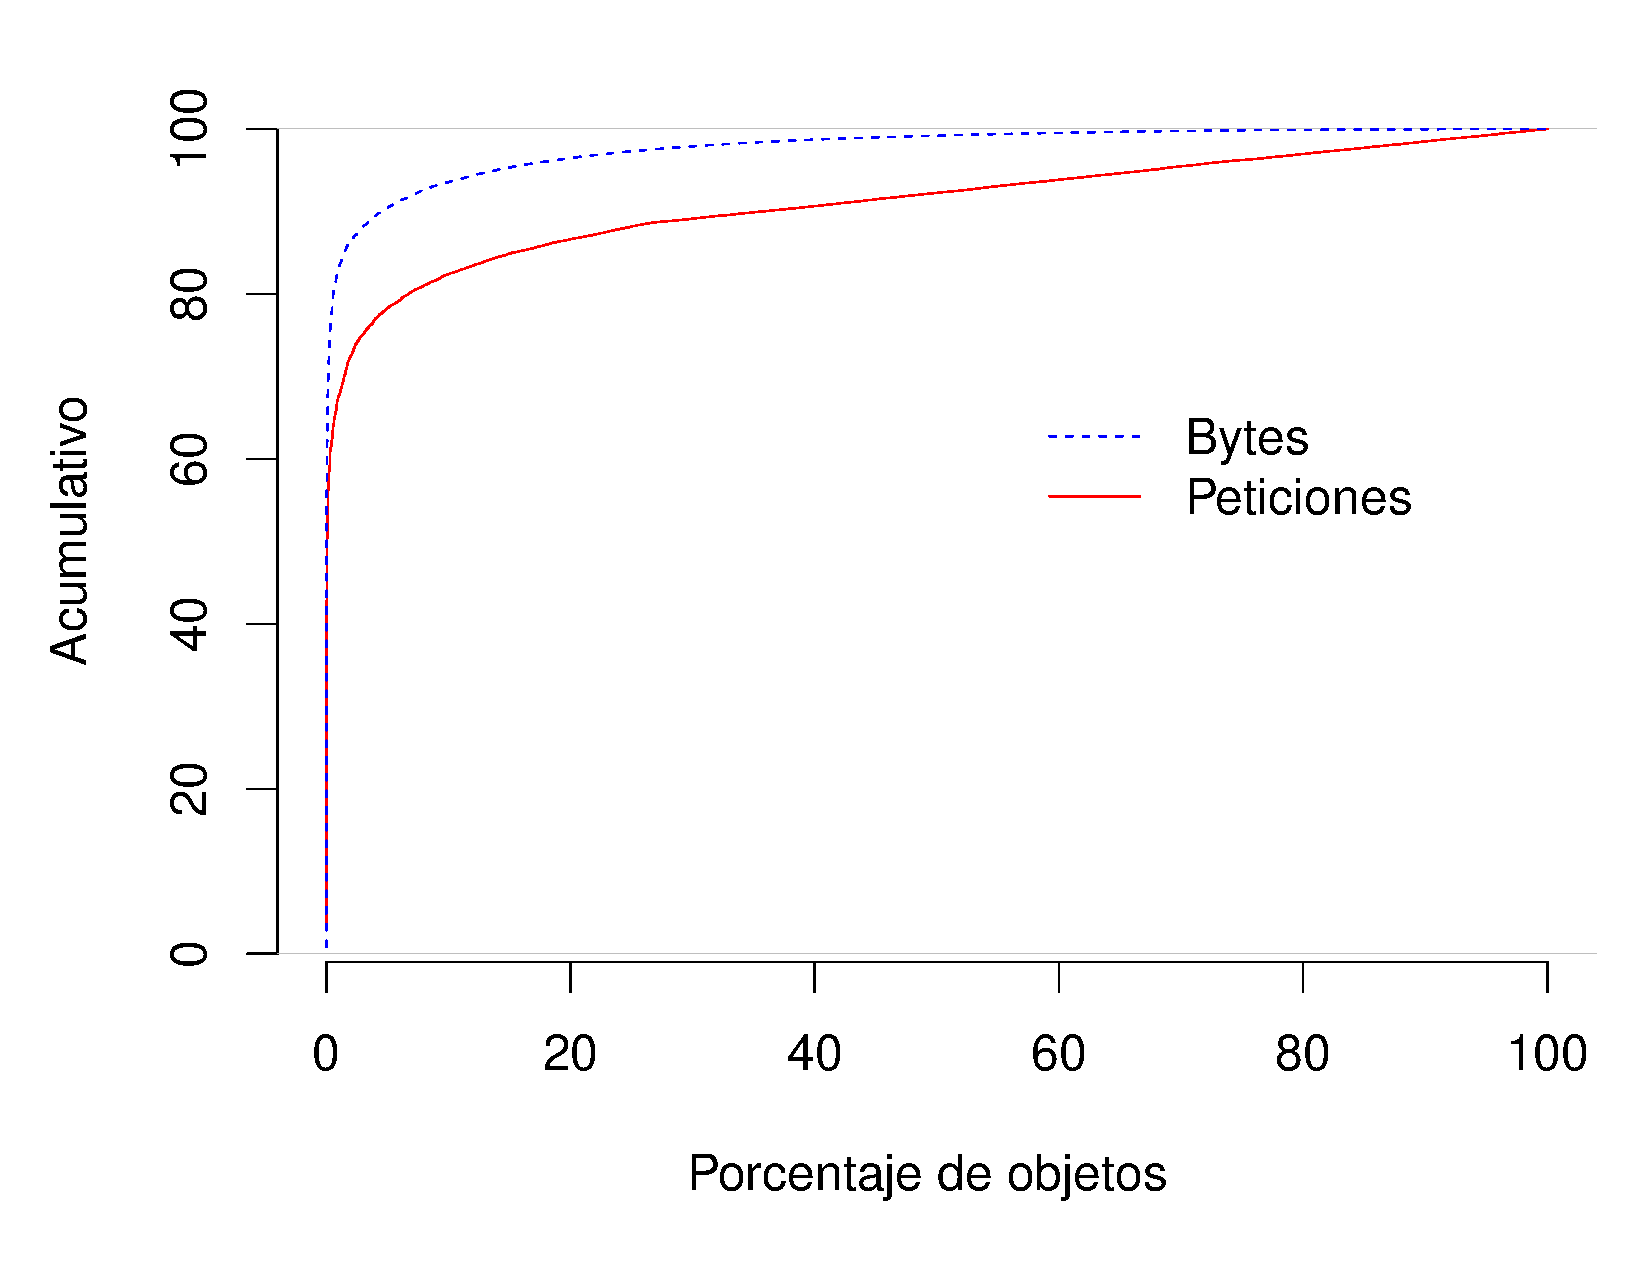
\includegraphics[scale=0.30]{figures/ObjectPopularityCum_full.pdf}
\caption{Frecuencia de referencia}
\label{fig:ObjectPopu}
\end{figure}
\begin{figure}[t]
\centering
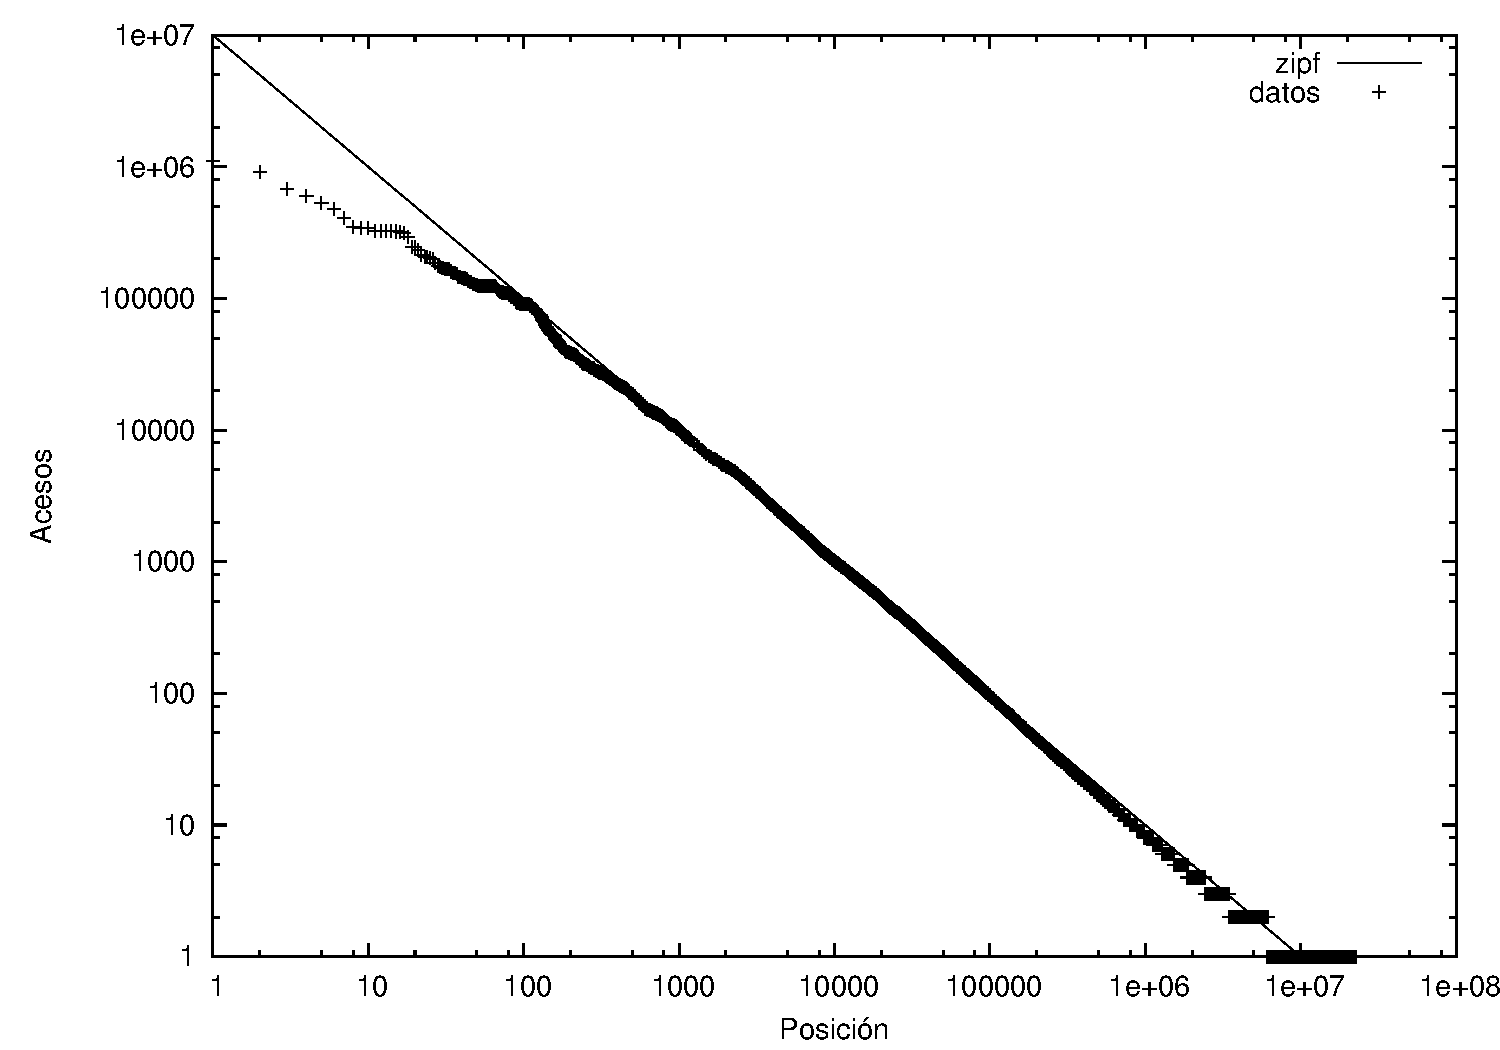
\includegraphics[scale=0.30]{figures/zipf.pdf} 
\caption{Frecuencia de referencia. Analisis zipf}
\label{fig:zipf}
\end{figure}

El que una porción tan pequeña de los objetos acumule la mayor parte de las referencias confirma que la técnica de caching es beneficiosa en la red de la universidad. Tal y como habíamos visto en la sección \ref{eficiencia} en los momentos de máxima demanda permite ahorrar un 15\% del tráfico saliente a Internet.

El segundo análisis determina la popularidad de los objetos. Los objetos únicos se encuentran ordenados una vez más en base al número de veces que son requeridos. Cada objeto tiene asignado un rango, donde el rango '1' se corresponde con el objeto único que presenta más referencias y el rango 'N' (asumiendo N objetos únicos) concedido al objeto único con el menor número de peticiones. La Figura \ref{fig:zipf} muestra el número total de accesos a cada uno de estos rangos, donde como se esperaba, el número de accesos decrece con la popularidad de los objetos únicos. Además, la distribución se puede estimar como una Zipf-like donde \emph{alpha} adquiere el valor de 1.

\subsection{Tiempo de sesión de los usuarios}
Debido a la dificultad de establecer cuando un usuario ha finalizado su sesión de navegación por la Web, hemos utilizado el método expuesto en el artículo \cite{adya2001analyzing}.

Este método consiste en intentar estimar cual es el tiempo de inactividad, a partir del cual, un usuario se considera que ha dejado de navegar por la Web. Para ello, hemos considerado cada IP como un usuario diferente y hemos variado el tiempo de inactividad entre 1 y 1000 segundos, contando en cada caso el número de nuevas sesiones. Hemos considerado que una sesión es nueva cuando el tiempo entre dos peticiones consecutivas es mayor que el tiempo de inactividad fijado.

Mediante este método hemos obtenido los resultados de la Figura \ref{fig:numberSessions}. Viendo este gráfico hemos llegado a pensar que el tiempo de inactividad ronda los 100 segundos, ya que es donde la curva deja de ser muy pronunciada y el número de sesiones parece estabilizarse.

\begin{figure}[]
\begin{center}
  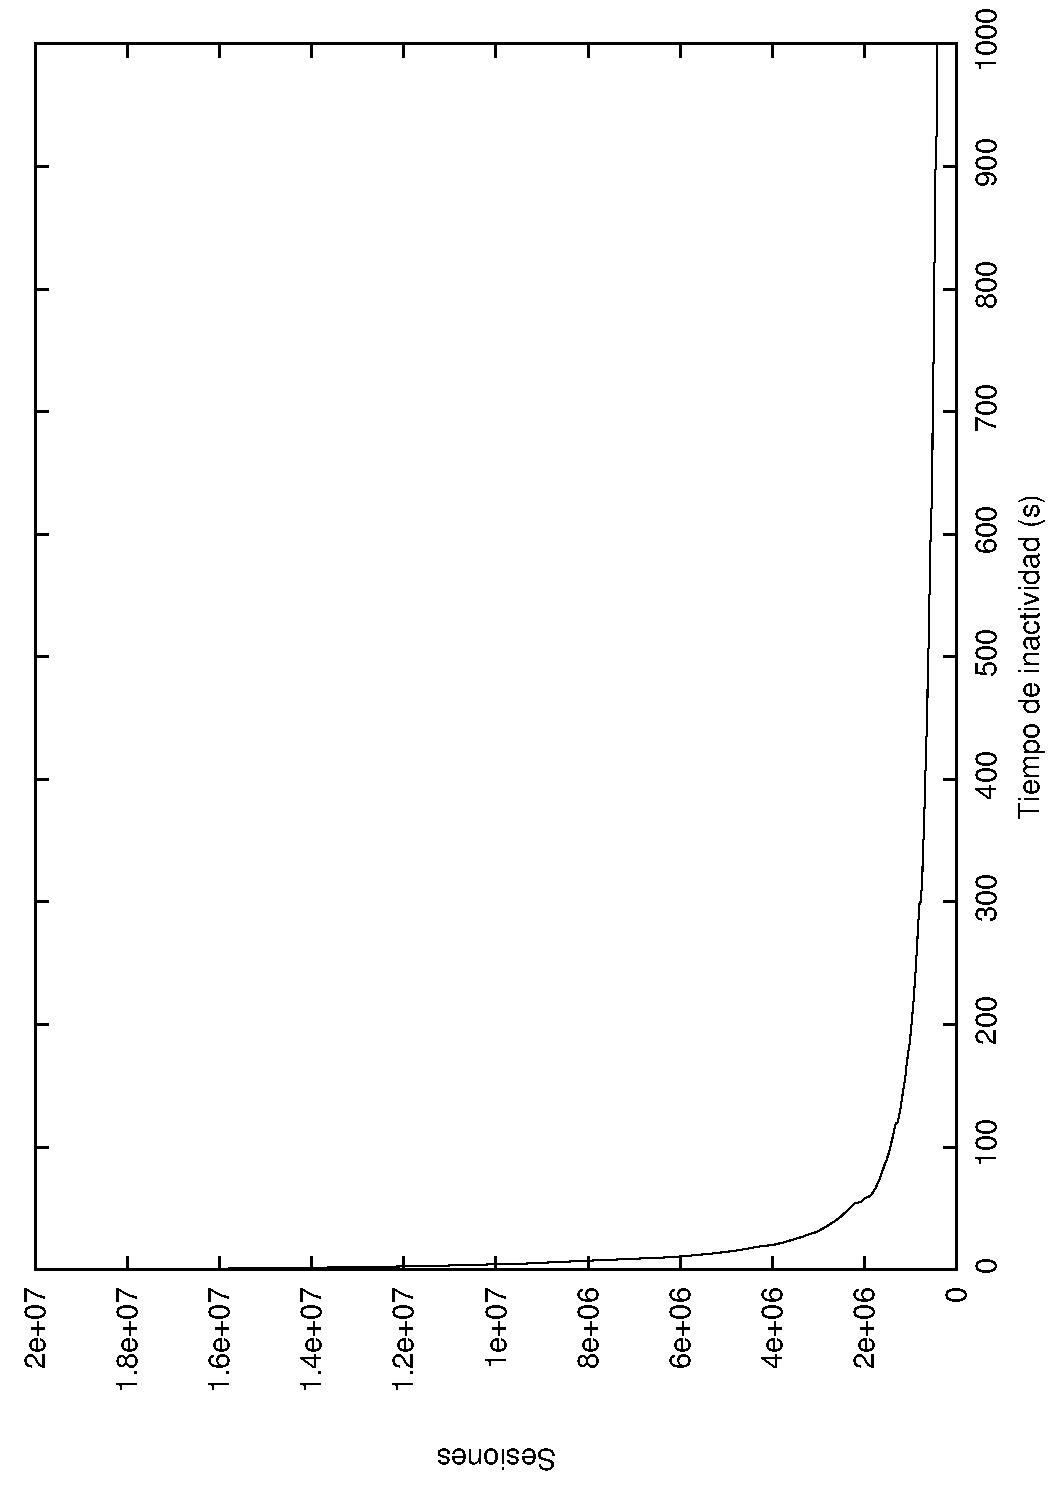
\includegraphics[scale=0.30,angle=-90]{figures/inactivityPeriod_full.pdf}
\end{center}
\caption{Número de sesiones vs. Periodos de inactividad} \label{fig:numberSessions}
\end{figure}

\begin{figure}[]
\begin{center}
  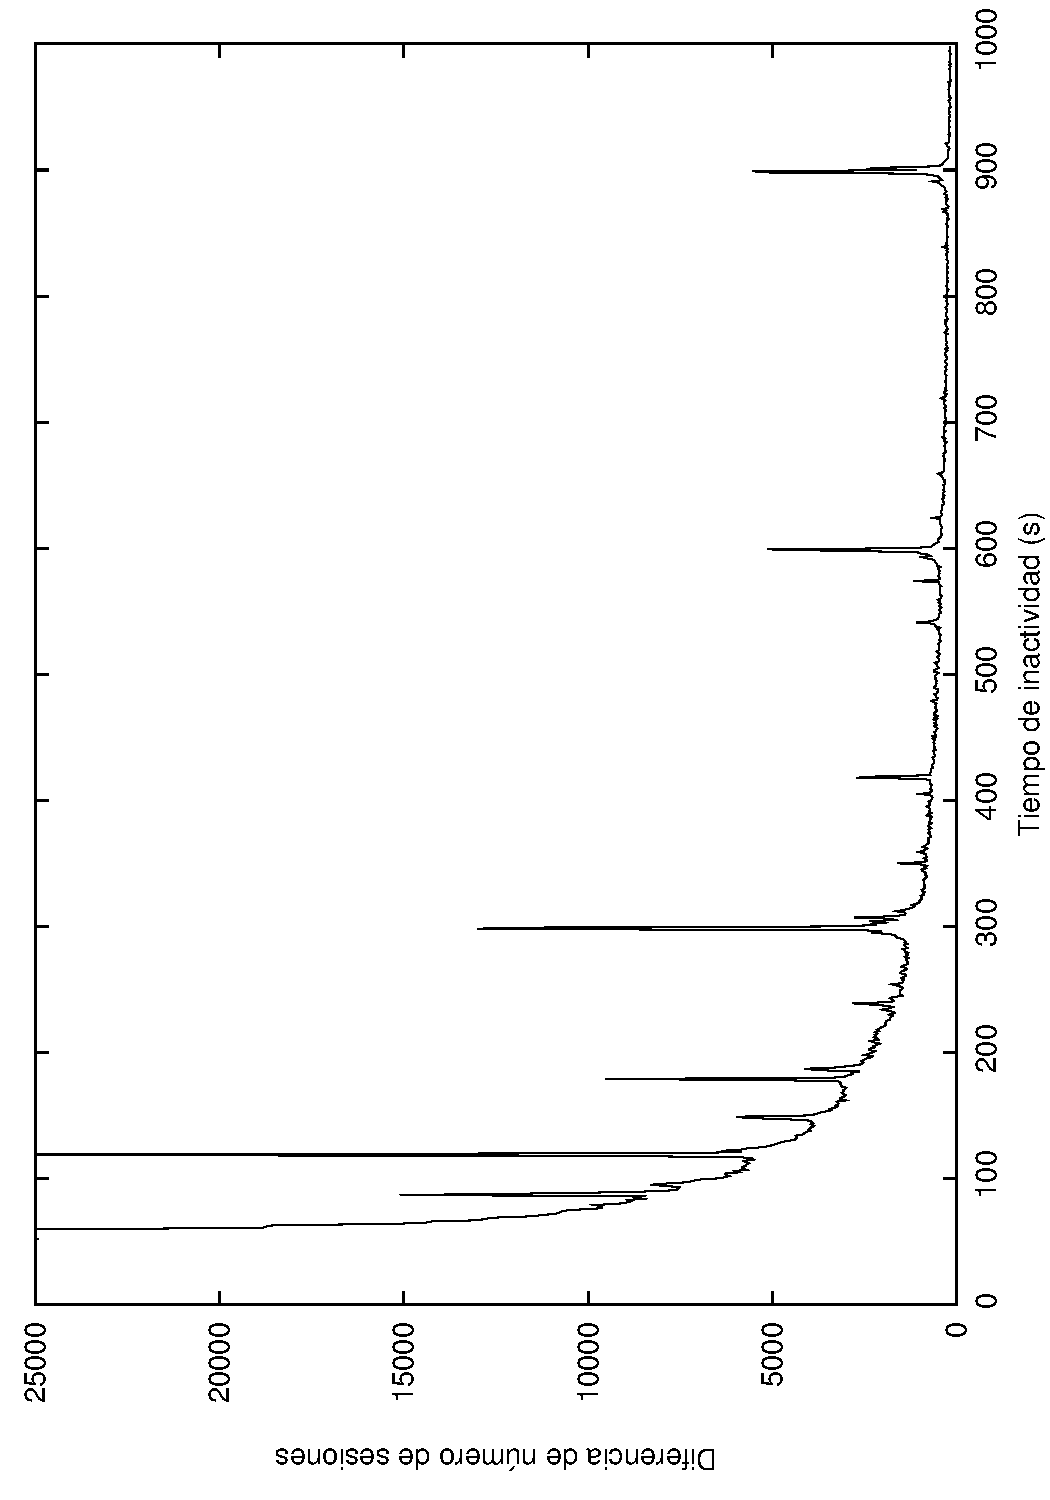
\includegraphics[scale=0.30,angle=-90]{figures/diffInactivitiPeriod_full.pdf}
\end{center}
\caption{Diferencia de sesiones} \label{fig:diffSessions}
\end{figure}

Para intentar corroborar esto, hemos estudiado alrededor de qué valores de tiempo hay más variabilidad de sesiones. Esto nos permite saber con más precisión cual es el tiempo de inactividad. Para ello, hemos obtenido la diferencia entre valores consecutivos de periodos de inactividad. Por ejemplo, hemos obtenido la diferencia entre las sesiones estimadas con un periodo de inactividad de 1 segundo y las sesiones estimadas con un periodo de inactividad de 2 segundos y así sucesivamente, obteniendo el gráfico de la Figura \ref{fig:diffSessions}.

En este gráfico hemos limitado los valores de diferencia entre número de sesiones a 25000 para poder apreciar con más claridad los picos. Como se puede observar, alrededor de los 100-120 segundos existe una gran diferencia entre el número de sesiones. Pero se pueden apreciar más diferencias, aunque no tan pronunciadas, a los 300, 600 y 900 segundos.

A la vista de los resultados y al contrario de lo que se afirma en el artículo \cite{adya2001analyzing}, el usuario de la red no tiene un tiempo de inactividad concreto a partir del cual podamos estimar la duración de las sesiones. Esta divergencia en los resultados puede ser debida simplemente a la diferencia entre los distintos tipos de usuarios que se estudian en ambos casos; ya que, en el artículo \cite{adya2001analyzing} se analiza el uso de la Web hecho por usuarios de dispositivos móviles. En cambio, en la universidad la mayoría de los equipos son ordenadores, tanto de sobremesa como portátiles.

\section{Conclusiones}
\label{conclusiones}

La técnica de caching es una de las más importantes en cuanto a la reducción de tráfico en la red. Consiste en almacenar objetos en caches cercanas a los clientes que los solicitan. Los aciertos en la cache eliminan la necesidad de acceder al servidor, reduciendo notablemente la demanda de ancho de banda y la latencia de la red a la vez que se mejora la disponibilidad del servidor. La técnica de caching se puede evaluar mediante la caracterización de la carga, ya que esta técnica explota propiedades específicas de los accesos para mejorar las prestaciones.
Mediante la caracterización de un sistema en el tiempo se pueden observar los cambios que el sistema ha sufrido. La carga objeto de análisis se ha obtenido de la Universidad Politécnica de Valencia durante 15 días.

La caracterización de la carga que se ha llevado a cabo en este trabajo ha estudiado en primer lugar la eficiencia del servidor proxy.
Los resultados han mostrado una gran diferencia entre los tiempos necesarios para resolver una petición a un objeto cacheado y no cacheado. Además, el máximo ancho de banda ahorrado se encuentra alrededor de 6Mbps, que resulta en un 15\% del ancho de banda en los momentos de máxima demanda. 

En segundo lugar se han analizado los códigos de respuesta del servidor, donde un 68\% de las peticiones resultan satisfactorias, mientras que un 19\% corresponde a peticiones a objetos no modificados. La mayoría del tráfico corresponde a peticiones satisfactorias, ya que las peticiones a objetos no modificados sólo transfieren las cabeceras HTTP.

En cuanto a los tipos de objetos que demandan los clientes, las imágenes han supuesto un 50\% del total de peticiones, mientras que los objetos HTML han obtenido un 26\%. Estos dos tipos de objetos representan un 21 y 9\% del total de GB de las peticiones respectivamente. Como se ha explicado anteriormente, el efecto se debe a que los vídeos y audios ocupan mayor tamaño que las imágenes y los HTML.

Por otra parte, el análisis del tamaño de los objetos únicos y solicitados  ha revelado que la mayoría de los objetos solicitados está entre 100B y 100KB y además se distribuyen conforme a una distribución de colas pesadas.

Los resultados de la evolución de la carga del servidor durante el día han mostrado el comportamiento de los usuarios de la universidad, donde la carga aunmenta durante las horas de trabajo. La tasa de aciertos se ha estabilizado entre un 30-40\% en los momentos de mayor carga.

El estudio de la localidad temporal ha confirmado que los patrones de referencia no son uniformes. Hemos distinguimos entre objetos extremadamente populares (1\% de objetos únicos suponen un 60\% de solicitudes), moderadamente populares (30\% de objetos únicos reciben un 90\% de solicitudes) y poco populares (10\% de objetos únicos). Por otra parte, hemos observado que el número de accesos a los objetos únicos decrece con la popularidad de los mismos y la distribución se puede aproximar a una Zipf-like donde \emph{alpha} adquiere el valor de 1.

Por último, en cuanto al tiempo de sesión de los usuarios, se ha estimado el tiempo de inactividad en unos 100 segundos, aunque los resultados obtenidos son variables debido al hecho de que el usuario de la universidad no tiene un tiempo de sesión concreto.

\nocite{*}
\bibliographystyle{Jornadas}

\begin{thebibliography}{1}


\bibitem{squid}
\newblock {\em Squid Internet Object Cache},
\newblock {\em available online at http://squid.nlanr.net}

\bibitem{mahanti}
A. Mahanti and M. Seltzer,
\newblock {Web Proxy Workload Characterization},
\newblock {\em Technical Report, Department of Computer Science, University of Saskatchewan},
\newblock {February, 1999}

\bibitem{duska}
B. Dushka, D. Marwood, and M. Feeley,
\newblock {The Measured Access Characteristics of World-Wide Web Client Proxy Caches},
\newblock {\em Proceedings of USENIX Symposium of Internet Technologies and Systems (USITS)},
\newblock {pp. 23-35, 1997}

\bibitem{Breslau}
L. Breslau, P. Cao, L. Fan, G. Phillips, and S. Shenker,
\newblock {Web Caching and Zipf-Like Distributions: Evidence and Implications},
\newblock {\em Proceedings of the IEEE Infocom},
\newblock {1999}

\bibitem{barish}
G. Barish and K. Obraczka,
\newblock {World Wide Web Caching: Trends and Techniques},
\newblock {\em  IEEE Communications Magazine},
\newblock {vol. 38, no. 5, pp. 178-184, 2000}

\bibitem{arlitt2}
M. Arlitt and C. Williamson,
\newblock {Internet Web Servers: Workload Characterization and Performance Implications},
\newblock {\em  IEEE/ACM Transactions on Networking},
\newblock {vol. 5, no. 5, pp. 631-645, 1997}

\bibitem{crovella}
M. Crovella and A. Bestavros,
\newblock {Self-Similarity in World Wide Web Traffic: Evidence and Possible Causes},
\newblock {\em  IEEE/ACM Transactions on Networking},
\newblock {vol. 5, no. 6, pp. 835-846, 1997}

\bibitem{adya2001analyzing}
Adya, A. and Bahl, P. and Qiu, L.,
  \newblock{Analyzing the browse patterns of mobile clients},
  \newblock{\em Proceedings of the 1st ACM SIGCOMM Workshop on Internet Measurement},
  \newblock{pp. 194, 2001}


\end{thebibliography}

\end{document}

\bibitem{arlitt}
M. Arlitt, R. Friedrich, and T. Jin,
\newblock {Workload Characterization of a Web Proxy in a Cable Modem Environment},
\newblock {\em ACM Performance Evaluation Review},
\newblock {vol. 27, no. 2, pp. 25-36, 1999}

